\documentclass{article}
\usepackage{amsmath, amssymb, cite, algorithmic, url, braket}
\usepackage{graphicx}
\usepackage{pythonhighlight}
\usepackage[margin=1.5cm]{geometry}
\usepackage[title]{appendix}
\usepackage{subfigure}
\usepackage{listings}
\usepackage{booktabs}

\graphicspath{{../pic/}}
\lstset{
language=[ANSI]{C},
showtabs=true,
tab=,
tabsize=2,
basicstyle=\ttfamily\footnotesize,%\setstretch{.5},
stringstyle=\color{stringcolour},
showstringspaces=false,
alsoletter={1234567890},
otherkeywords={\%, \}, \{, \&, \|},
keywordstyle=\color{keywordcolour}\bfseries,
upquote=true,
morecomment=[s]{/*}{*/},
commentstyle=\color{commentcolour}\slshape,
literate=*%
{=}{{\literatecolour=}}{1}%
{-}{{\literatecolour-}}{1}%
{+}{{\literatecolour+}}{1}%
{*}{{\literatecolour*}}{1}%
{!}{{\literatecolour!}}{1}%
{[}{{\literatecolour[}}{1}%
{]}{{\literatecolour]}}{1}%
{<}{{\literatecolour<}}{1}%
{>}{{\literatecolour>}}{1}%
% {>>>}{\pythonprompt}{3}%
,%
frame=trbl,
rulecolor=\color{black!40},
backgroundcolor=\color{white},
breakindent=.5\textwidth,frame=single,breaklines=true
}

\begin{document}
\title{DSP Homework}
\author{Xu, Minhuan}
\maketitle
\tableofcontents
\begin{abstract}
This week, we experienced the scenery of deserts and grasslands. Then, in the second section, I derived the formula for IDFT from DFT. In the third section, I found a way to find analog spectral components in DFT by rewriting the formula for DTFT. Finally, I \emph{assemble} the codes shown in class to complete the task of comparing the running speed. But, by using Matplotlib, I drew a graph to compare the speed of different code implementations of DFT.
\end{abstract}

\section{Videos}
\subsection{Our Planet}
From this video, we can see how ecosystems are connected, from creatures in the desert to creatures in the grasslands, whether it is cormorants or bison, whether it is cheetahs or tigers, they are all on the same earth. Just like the relationship between Alcon Blue, ants, and gentian, we humans and animals should also be interdependent. Of course, we humans also have the obligation and responsibility to protect this earth, so whether it is poaching, endless expansion of agriculture, or other behaviors that destroy wildlife habitats should be controlled, which is indeed our responsibility.

\subsection{My Thoughts}
We've been learning about the water cycle on Earth, where water evaporates from the ground, is carried around the world by the wind, and then falls to all corners of the earth in the form of rain. This kind of air water cycle is dependent on the atmosphere and its flow, that is, the wind. It is carried out, and in the video, it is specifically mentioned that the dust in the desert is transported to the sea through the wind to provide nutrients. I think that's why I love this documentary

\section{IDFT}
To derive the IDFT formula, we only should derive the expression of $A^{-1}$. And since $A$ can be expressed as below
$$
\begin{bmatrix}
 1 & 1 & 1 & \cdots & 1 \\
 1 & w^1 & w^2 & \cdots & w^{N - 1} \\
 1 & w^2 & w^4 & \cdots & w^{2(N - 1)}\\ 
 \vdots & \vdots & \vdots& \ddots & \vdots\\
 1 & w^{2(N - 1)} & w^{4(N - 1)} & \cdots & w^{(N - 1)^2}
 \end{bmatrix}
$$
we note rows in A as $\alpha_i$, and rewrite it as below
$$
A = 
\begin{bmatrix}
\alpha_0 \\ \alpha_1 \\ \alpha_2 \\ \vdots \\ \alpha_{N - 1}
 \end{bmatrix} 
$$
See $\alpha_i \cdot \alpha_j^H$, if $i \neq j$, we let $\lambda = i - j \in (0, N)$, and
\begin{equation}
\begin{aligned}
    \alpha_i \cdot \alpha_j^H &= \begin{bmatrix}
    1 & w^i & w^{2i} & w^{3i} & \cdots & w^{(N - 1)i}
     \end{bmatrix}
     \cdot
     \begin{bmatrix}
    1 \\ w^j \\ w^{2j} \\ w^{3j} \\ \vdots \\ w^{(N - 1)j}
     \end{bmatrix}\\
     &= 1 + w^{\lambda} + w^{2 \lambda} + \cdots + w^{(N - 1) \lambda}\\
     &= \frac{1 - w^{N \lambda}}{1 - w^{\lambda}}\\ 
     &= \frac{1 - e^{j 2\pi\lambda} \quad (= 0)}{1 - e^{-j\frac{2\pi}{N}\lambda} \quad (\neq 0)}\\ 
     &= 0
\end{aligned}
\label{eq:inj}
\end{equation}
If $i = j$, we have
\begin{equation}
    \alpha_i \cdot \alpha_j^H = 1 + w^{0} + w^{2 \times 0} + \cdots + w^{(N - 1) \times 0} = N
    \label{eq:ij}
\end{equation}
So, conclude (\ref{eq:inj}) and (\ref{eq:ij}), we have
\begin{equation}
    \alpha_i \cdot \alpha_j^H =
    \begin{cases}
        0 & \text{if } i \neq j \\ 
        N & \text{if } i = j
    \end{cases}
\label{eq:multi_ij}
\end{equation}
Therefore, see $A \cdot A^H$
\begin{equation}
\begin{aligned}
    A \cdot A^H &= 
    \begin{bmatrix}
        \alpha_0 \\ \alpha_1 \\ \alpha_2 \\ \vdots \\ \alpha_{N - 1}
    \end{bmatrix}
    \cdot
    \begin{bmatrix}
        \alpha_0^H & \alpha_1^H & \alpha_2^H & \cdots & \alpha_{N - 1}^H
    \end{bmatrix} \\ 
    &= N \cdot 
    \begin{bmatrix}
        \alpha_0 \cdot \alpha_0^H & \alpha_0 \cdot \alpha_1^H & \cdots & \alpha_0 \cdot \alpha_{N - 1}^H \\ 
        \alpha_1 \cdot \alpha_0^H & \alpha_1 \cdot \alpha_1^H & \cdots & \alpha_1 \cdot \alpha_{N - 1}^H \\ 
        \vdots & \vdots & \ddots & \vdots \\ 
        \alpha_{N - 1} \cdot \alpha_0^H & \alpha_{N - 1} \cdot \alpha_1^H & \cdots & \alpha_{N - 1} \cdot \alpha_{N - 1}^H
    \end{bmatrix} \\
    &= N \cdot 
    \begin{bmatrix}
        1 & 0 & \cdots & 0 \\ 
        0 & 1 & \cdots & 0 \\ 
        \vdots & \vdots & \ddots & \vdots \\ 
        0 & 0 & \cdots & 1
    \end{bmatrix} \\
    &= N \cdot I
\end{aligned}
\label{eq:AAH}
\end{equation}
If we multiply $A^{-1}$ in both side of (\ref{eq:AAH}), we have
\begin{equation}
    A^{-1} = \frac1N A^H
\label{eq:A-1}
\end{equation}
Therefore, IDFT formula can be expressed as below
\begin{equation}
    \begin{aligned}
        x &= A^{-1} \tilde{x}\\ 
        &= \frac1N A^H \tilde{x} \\ 
        &= \frac{1}{N} (A \tilde{x}^H)^H \\ 
        &= \frac{1}{N} \sum^{N - 1}_{k = 0} \tilde{x}(k)e^{j2\pi kn /N}
    \end{aligned}
\end{equation}
Also, a more symmetric definition is as below
$$
    \tilde{x}(k) = \frac{1}{\sqrt{N}} \sum_{n = 0}^{N - 1} x(n) e^{-j 2\pi kn/N}
$$
$$
    x(n) = \frac{1}{\sqrt{N}} \sum_{k = 0}^{N - 1} \tilde{x}(k) e^{j 2\pi kn/N}
$$
\section{Find Analog Spectrum Value in DFT}
The DTFT formula can be rewritten as below
\begin{equation}
\begin{aligned}
\tilde{x}_s(f) &= \mathcal{F} \left[ x_s(t) \right] \\ 
&= \mathcal{F} \left[ x_a(t) \times s(t) \right] \\ 
&= \tilde{x}_a(f) *\tilde{s}(f) \\ 
&= \tilde{x}_a(f) * \left[ f_s \sum_n \delta(f - nf_s) \right] \\
&=f_s \cdot \sum_n \tilde{x}_a(f - nf_s) \\
\end{aligned}
\label{eq:dtft_rewrite}
\end{equation}
To make the frequency discrete, we should do sampling in frequency domain. The period of (\ref{eq:dtft_rewrite}) is $f_s$, so we make the analog frequency be $f = f_s \cdot \frac k N$.

Therefore, we have
\begin{equation}
\begin{aligned}
\tilde{x}(\frac{k\cdot f_s}{N}) &= f_s \cdot \sum_n \tilde{x}_a[f_s \cdot \frac kN - f_s \cdot n] \\ 
&= f_s \cdot \sum_n \tilde{x}_a[f_s(\frac kN - n)]
\end{aligned}
\label{eq:dtft_rewrite_2}
\end{equation}
In order to compute the exact value of $\tilde{x}_a(f)$ for $f = 3010.3 ~\mathrm{Hz} $, we should make $f_s(\frac kN - n) = 3010.3 ~\mathrm{Hz}$ in (\ref{eq:dtft_rewrite_2}). Usually, we know that $f_s > B$ where $B$ is the bandwidth of $x_a(t)$, so $n$ must be $0$, therefore, in order to compute the exact frequency spectrum value, we only should to compute: 
$$
f_s\cdot \frac kn = 3010.3 ~\mathrm{Hz}
$$


\section{Comparison of Codes Running Speed}
Assuming $N$ is the total number of the sampling points, I drew a picture of how much time it takes for 3 methods to do the calculations. The x-axis is $\mathrm{Log}N$, and the y-axis is Time $t$. See Fig.~\ref{fig:speedtest}

\begin{figure}[!h]
    \centering
    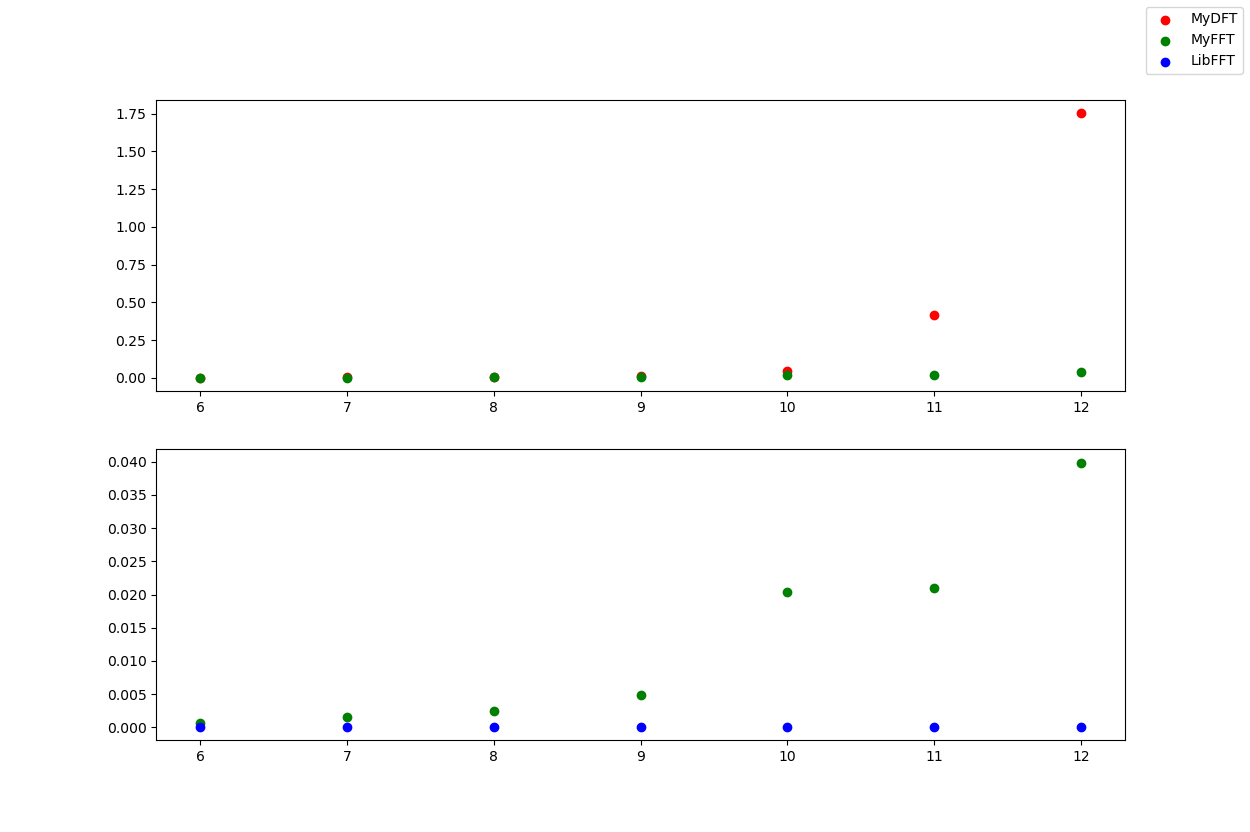
\includegraphics[width=5 in]{../pic/speedtest.png}
    \caption{Comparison of the Codes Running Speed}
    \label{fig:speedtest}
\end{figure}

\newpage

\bibliographystyle{ieeetr}
\bibliography{../bib/database}

\begin{appendices}
\section{Code Listing}
\begin{python}
import numpy as np
import time
from matplotlib import pyplot as plt

def dft(x):
    N = len(x)
    xt = np.matmul(
        np.exp(-1j * 2 * np.pi * np.matmul(np.arange(N).reshape(N, 1), np.arange(N).reshape(1, N)/N)),
        x
        )
    return xt

def idft(xt):
    return np.conj(dft(np.conj(xt))) / N

def fft(x):
    N = len(x)
    if N == 1:
        return x
    else:
        x0, x1 = x[::2] , x[1::2]
        xt0 = fft(x0)
        xt1 = fft(x1)
        tmp = np.exp(-1j*2*np.pi*np.arange(N/2)/N) * xt1
        xt = np.concatenate([xt0 + tmp, xt0 - tmp])
    return xt

def ifft(xt):
    return np.conj(fft(np.conj(xt))) / N

def test(m):
    x = np.random.rand(2**m)

    # MyDFT
    st1 = time.time()
    y1 = dft(x)
    et1 = time.time()
    # xx1 = idft(y1)

    # MyFFT
    st2 = time.time()
    y2 = fft(x)
    et2 = time.time()
    # xx2 = idft(y2)

    # LibFFT
    st3 = time.time()
    y3 = np.fft.fft(x)
    et3 = time.time()
    # xx3 = idft(y3)

    # err1 = xx1 - x
    # err2 = xx2 - x
    # err3 = xx3 - x

    t1 = et1 - st1
    t2 = et2 - st2
    t3 = et3 - st3
    
    return t1, t2, t3


M = [i for i in range(6, 13)]
T1 = []
T2 = []
T3 = []
for m in M:
    tmp1, tmp2, tmp3 = test(m)
    T1.append(tmp1)
    T2.append(tmp2)
    T3.append(tmp3)

fig = plt.figure()
plt.xlabel('LogN')
plt.ylabel('Time')
plt.subplot(211)
plt.scatter(M, T1, label='MyDFT', c='r')
plt.scatter(M, T2, label='MyFFT', c='g')
plt.subplot(212)
plt.scatter(M, T2, c='g')
plt.scatter(M, T3, label='LibFFT', c='b')
fig.legend()
plt.show()
\end{python}
\end{appendices}

\end{document}